\documentclass{handout}

\SetInstructor{ Lt Col James Phillips}
\SetCourseTitle{ECE231: Electrical Circuits and Systems I}
\SetSemester{Spring 2016}
\SetHandoutTitle{Lecture 2: Resistors, Sources, Switches, KCL, KVL}
%\SetDueDate{1 Jan 2016}
%\ShowAllBlanks

\showsoln \setsolncolor{red}

\begin{document}
\maketitle

\textbf{Upcoming events}

\begin{itemize}
\item Skills review due today
\item HW \#1 (lessons 1 \& 2) due Lesson 3
\item HW \# 2 (lessons 3 \& 4) due Lesson 5
\item Problem Set \# 1 due Lesson 5
\item Quiz \# 1 during Lesson 6
\end{itemize}

\textbf{OBJECTIVES:}
\begin{enumerate}
\item Introduce sources \& switches
\item Introduce the concept of {\em Nodes} \& {\em Loops}
\item Learn and apply Kirchhoff's Voltage \& Current Laws (KVL \& KCL)
\item Solve circuits using KCL, KVL and Ohm's Law

\end{enumerate}

\textbf{READING}
\begin{description}
\item [Required:] Textbook, sections 2.1--2.2, pages 15--26
\item [Optional:]None
\end{description}

\textbf{HOMEWORK}
\begin{description}
\item [Required textbook problems]: 2.5, 2.15, 2.17, 2.23 --- Due Lesson 3
\item [Recommended textbook problems]: 2.6, 2.16, 2.22
\item[Other]: Instructor Created Problem Set 1 --- Due Lesson 5
\end{description}

\section{A quick review of Resistors}
We introduced resistors in last class along with Ohm's Law. Figure \ref{fig: Resistor_VI_Relationship} shows the resistor current--voltage ($i$--$v$) relationship.  We will develop $i$--$v$ relationships for other devices as we go along.

\begin{figure}[h b]
\centering
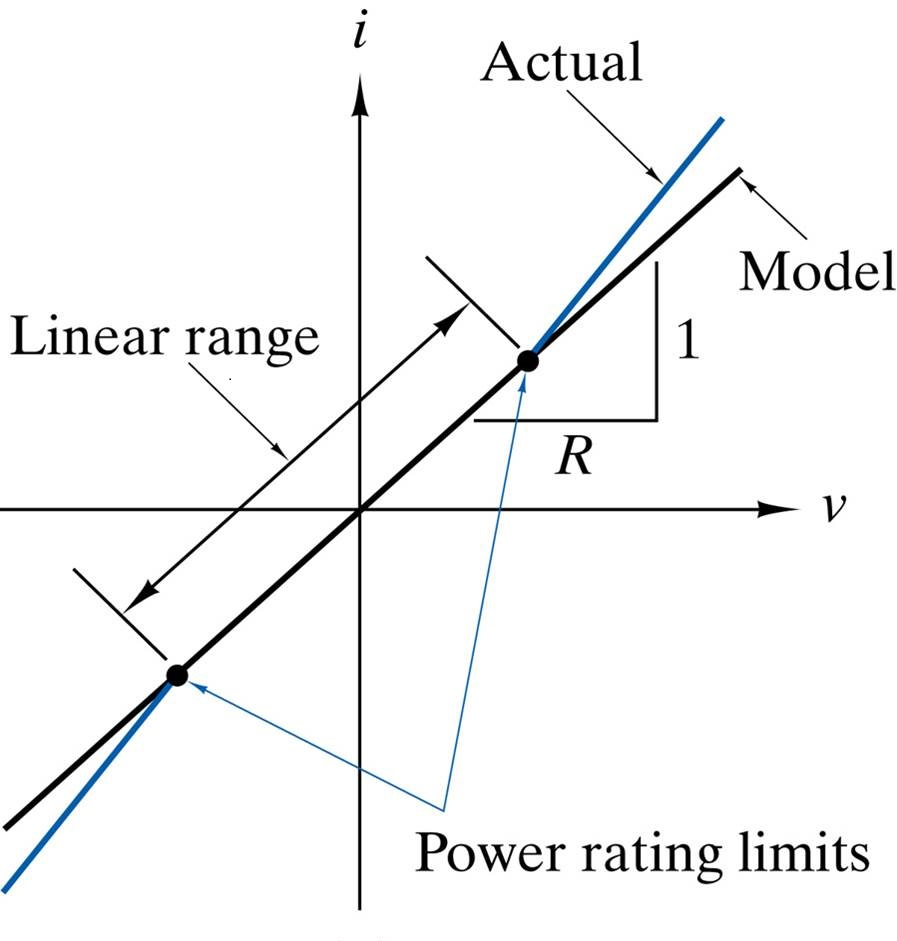
\includegraphics[width=0.25\textwidth]{Resistor_VI_Relationship.jpg}
\caption{Resistor VI relationsip}
\label{fig: Resistor_VI_Relationship}
\end{figure}

\section{Open Circuits, Short Circuits and Switches}
\begin{description}
\item [Open Circuits] are a ''broken'' paths that no current can flow through.  Voltage can exist across an open circuit.  Open circuits can be modeled as an $\infty$ resistance.  An open circuit is shown in Figure \ref{fig: Open_and_Short_Circuits}(a).
\item [Short Circuits] are closed paths that have zero resistance.  A short circuit has zero voltage across it. A short circuit is shown in Figure \ref{fig: Open_and_Short_Circuits}(b).
\item [Ideal Switchs] are devices that can create an open or short circuit depending on the switch position. See Figure \ref{fig: Switch} for schematics and  $i$--$v$ characteristics of open and closed {\em ideal} switches.
\end{description}

\begin{figure}[h b t]
\centering
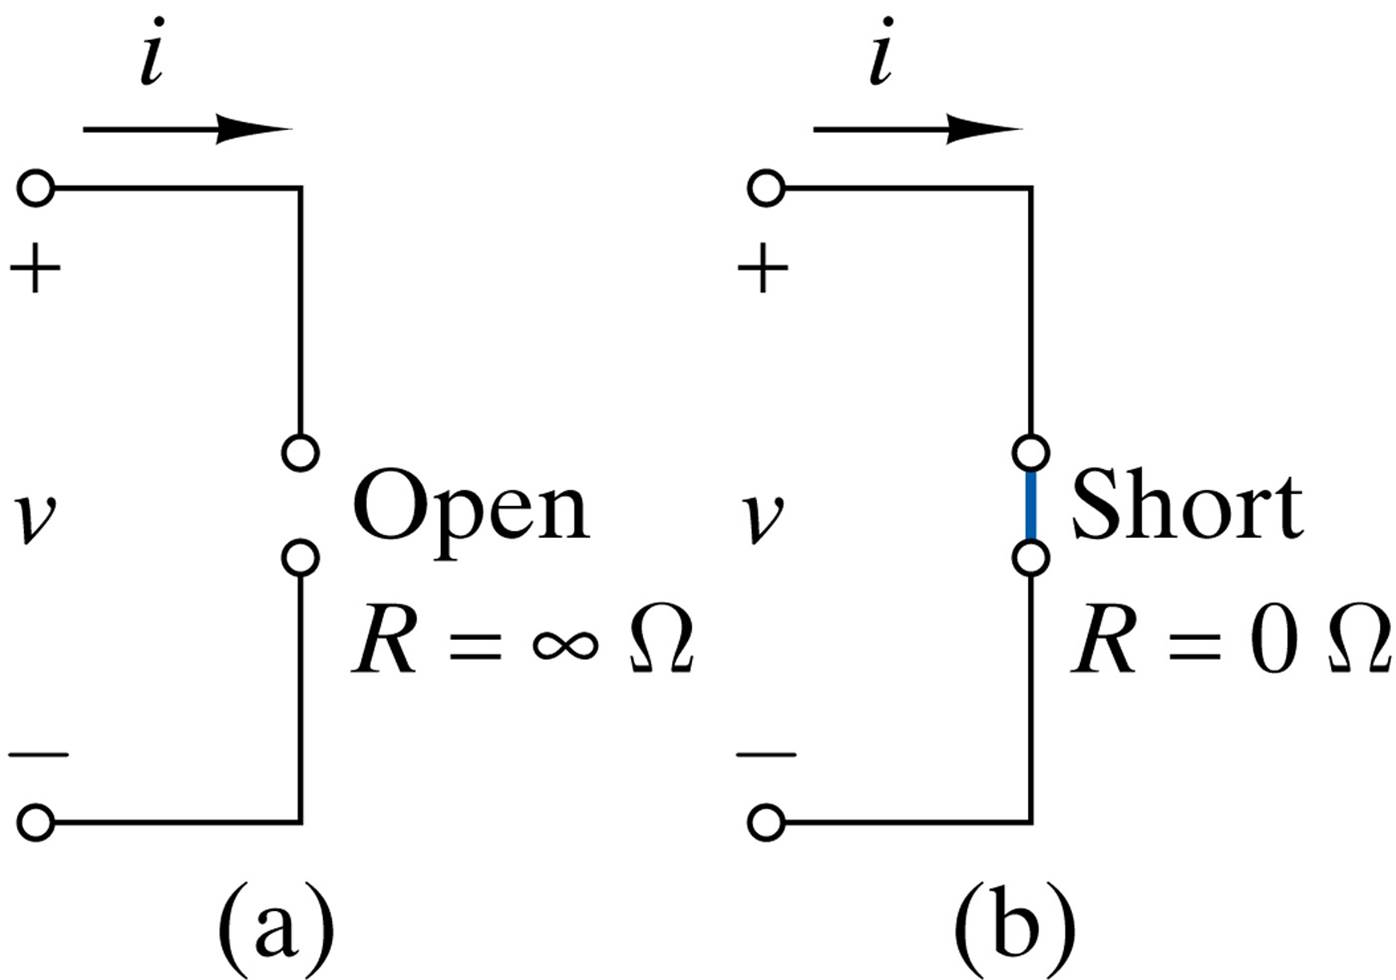
\includegraphics[width=0.5\textwidth]{Open_and_Short_Circuits.jpg}
\caption{Schematic of (a) an open circuit and (b) a short circuit}
\label{fig: Open_and_Short_Circuits}
\end{figure}

\begin{figure}[h b t]
\centering
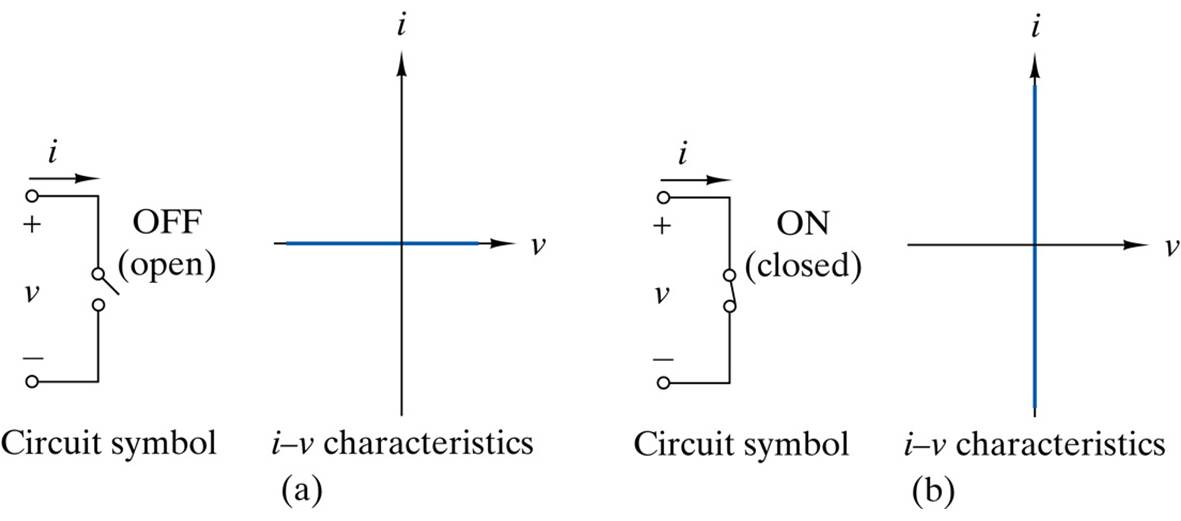
\includegraphics[width=0.75\textwidth]{Switch.jpg}
\caption{Schematic \& $i$--$v$ relationship of (a) an open switch (open circuit) and (b) a closed switch (short circuit)}
\label{fig: Switch}
\end{figure}

\newpage

\section{Ideal Sources}
For now we will deal with only ideal voltage sources and ideal current sources.  What do we mean by ideal?

\soln{1.0in}{The source provides the same current or voltage output independent of the load it is connected to.  Another way of saying this is that the  $i$--$v$ characteristic is always a constant.  For a current source, $i(v)=constant$. for a voltage source, $v(i)=constant$.}

Figure \ref{fig: Ideal_Voltage_Source} shows schematics of ideal voltage sources and the  $i$--$v$ characteristic.

\begin{figure}[h b t]
\centering
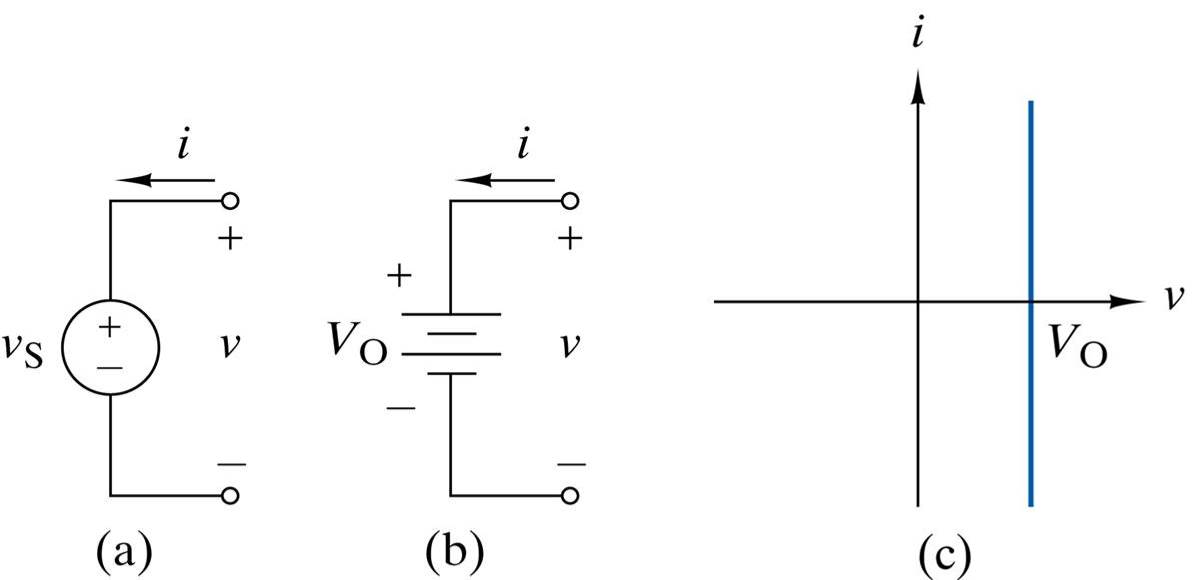
\includegraphics[width=0.85\textwidth]{Ideal_Voltage_Source.jpg}
\caption{(a) An ideal voltage source,  (b) an ideal battery, and (c) their $i$--$v$ characteristic}
\label{fig: Ideal_Voltage_Source}
\end{figure}

Figure \ref{fig: Ideal_Current_Source} shows the schematics of an ideal current sources and the  $i$--$v$ characteristic.

\begin{figure}[h b t]
\centering
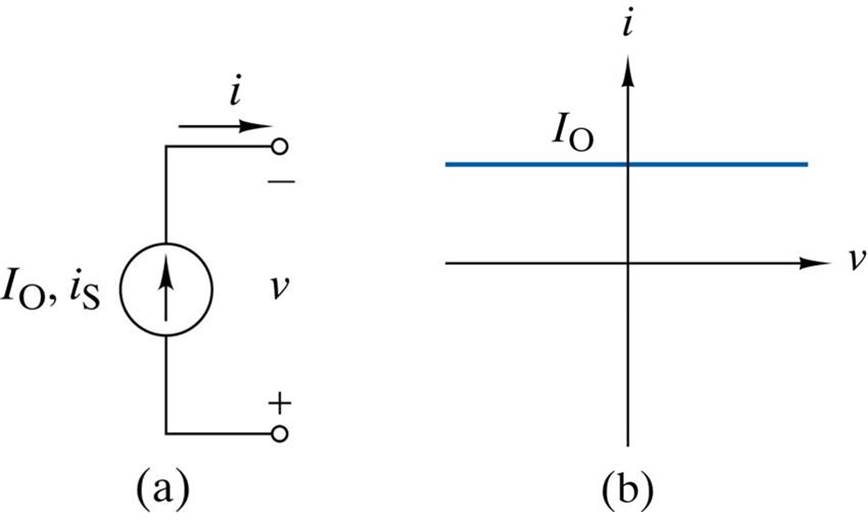
\includegraphics[width=0.5\textwidth]{Ideal_Current_Source.jpg}
\caption{(a) An ideal current source, and  (b) its $i$--$v$ characteristic}
\label{fig: Ideal_Current_Source}
\end{figure}

\textbf{Thought Question:} Can a car battery be modeled as an ideal voltage source? Why or why not?

\soln{1.5in}{
No.  When you start your car, starter draws very high current from the battery (around 100-250A).  When the current draw is this high, the voltage from the battery will decrease to 8-10V.  Since the voltage is not constant, but rather is dependent on current, it is not an ideal source
}

\newpage

\section{Nodes}

What is a \textbf{node}?

\soln{3in}{
\begin{enumerate}
\item A node is the junture of {\em two or more} devices
\item The node includes all the wire running between devices
\end{enumerate}
}

You need to be able to count nodes in a circuit.  The easiet way to do that is to ''erase'' all the devices, but leave the wire.  The ''clumps'' of wire left behind are your nodes. Figure \ref{fig: CountingNodes} demonstrates this procedure.

\begin{figure}[h b t]
\centering
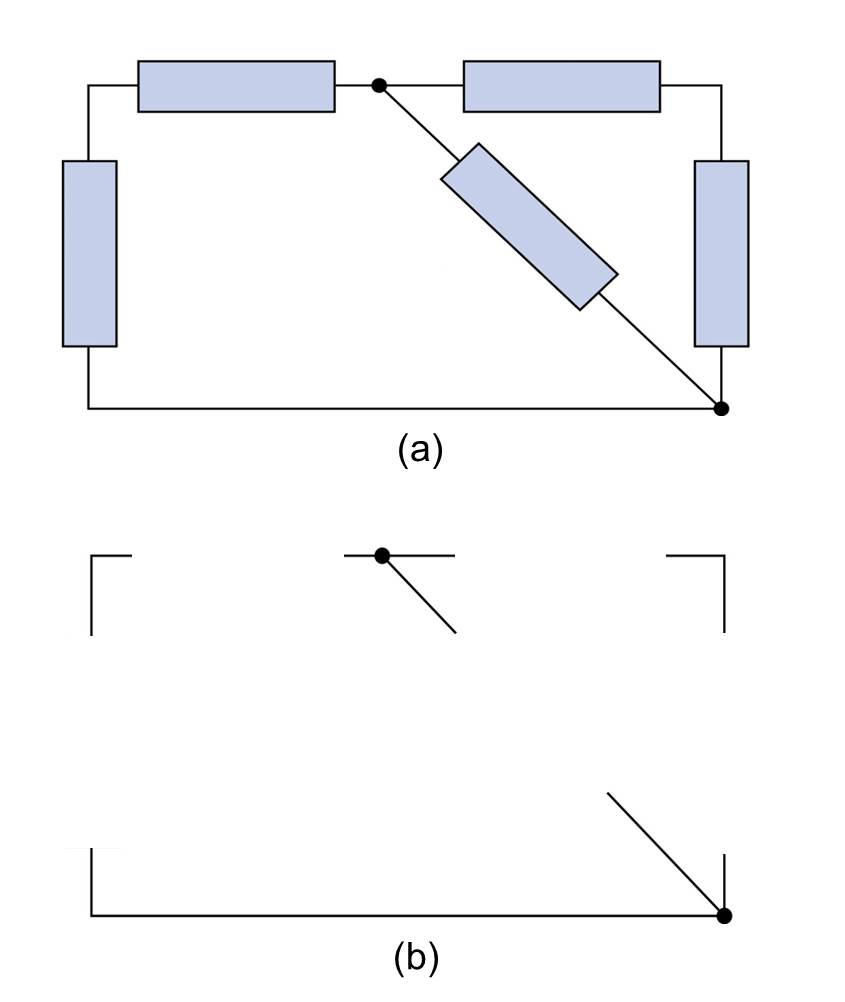
\includegraphics[width=0.4\textwidth]{CountingNodes.jpg}
\caption{(a) A simple circuit,  (b) the same circuit with devices removed leaving only the 4 nodes}
\label{fig: CountingNodes}
\end{figure}

\newpage

\section{Loops}

What is a \textbf{loop}?

\soln{2in}{
\begin{enumerate}
\item A loop is a closed path through a circuit
\item A loop cannot pass through any node twice; other than starting and finishing at the same node (which is the definition of a closed path)
\end{enumerate}
}

You also need to be able to identify and count loops in a circuit. See  Figure \ref{fig: SimpleLoopCounting} for a simple example and Figure \ref{fig: ComplicatedLoopCounting} for a more complicated example.

\begin{figure}[h b t]
\centering
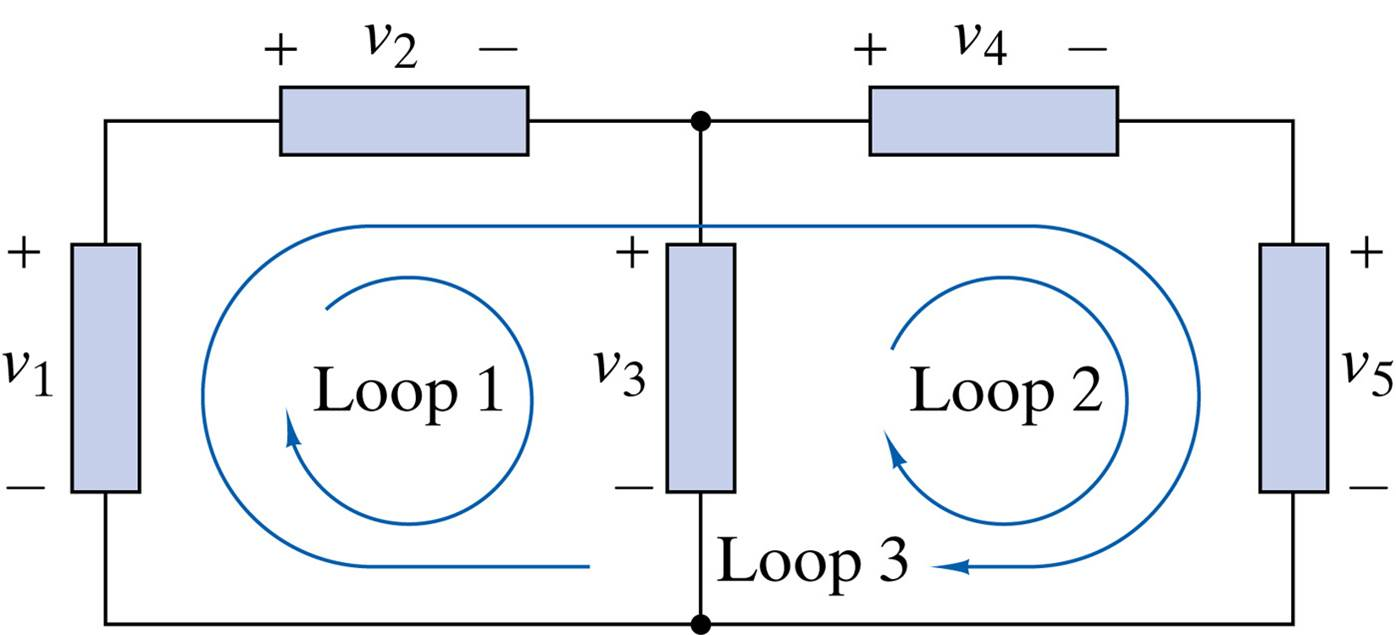
\includegraphics[width=0.5\textwidth]{SimpleLoopCounting.jpg}
\caption{Example circuit with 3 loops}
\label{fig: SimpleLoopCounting}
\end{figure}

\begin{figure}[h b t]
\centering

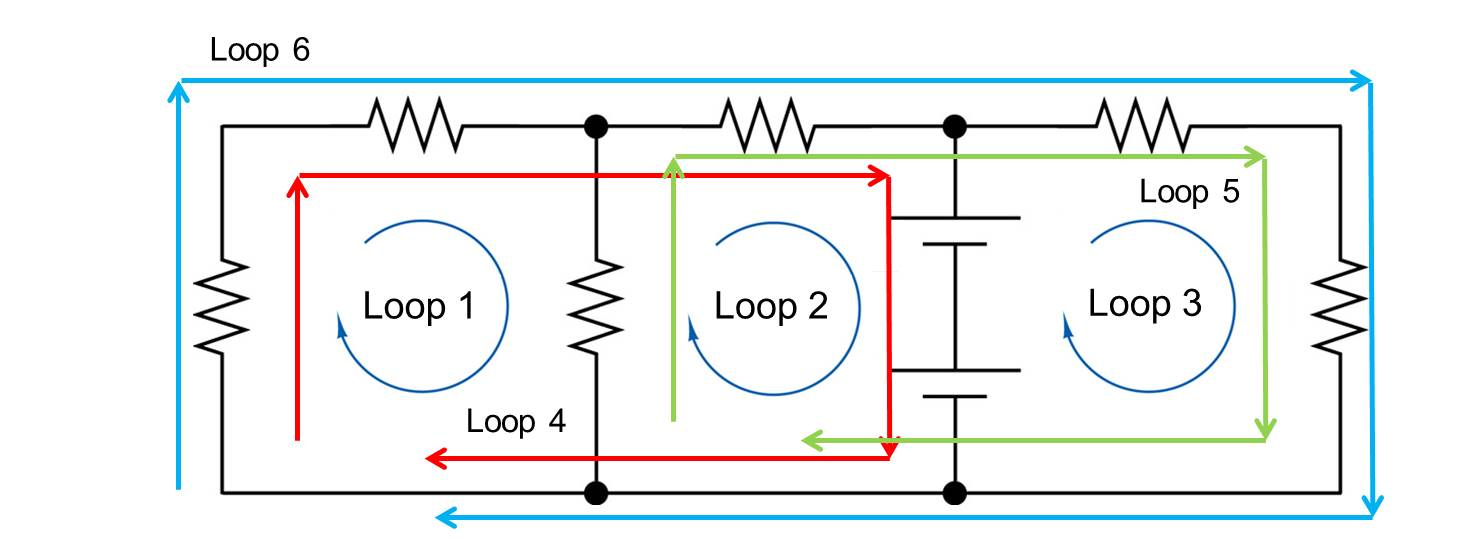
\includegraphics[width=0.85\textwidth]{ComplicatedLoopCounting.jpg}
\caption{Example circuit with 6 loops}
\label{fig: ComplicatedLoopCounting}
\end{figure}

\newpage

\section{Kirchhoff's Current Law (KCL)}
Kirchhoff's Current Law in words

\soln{2.5in}{
\begin{enumerate}
\item Algebraic sum of all currents at a node equals zero
\item Sum of currents entering a node equals the sum of currents leaving the node
\item Goes-intas = Goes-outas
\end{enumerate}
}

KCL in mathematics

\begin{equation}
\sum_{Node} i = 0 
\end{equation}

\begin{equation}
\sum i_{in} = \sum i_{out}
\end{equation}

\begin{equation}
\sum goesintas = \sum goesoutas
\end{equation}

Write a KCL equation for the center node in Figure \ref{fig: KCL}
\begin{figure}[h b t]
\centering
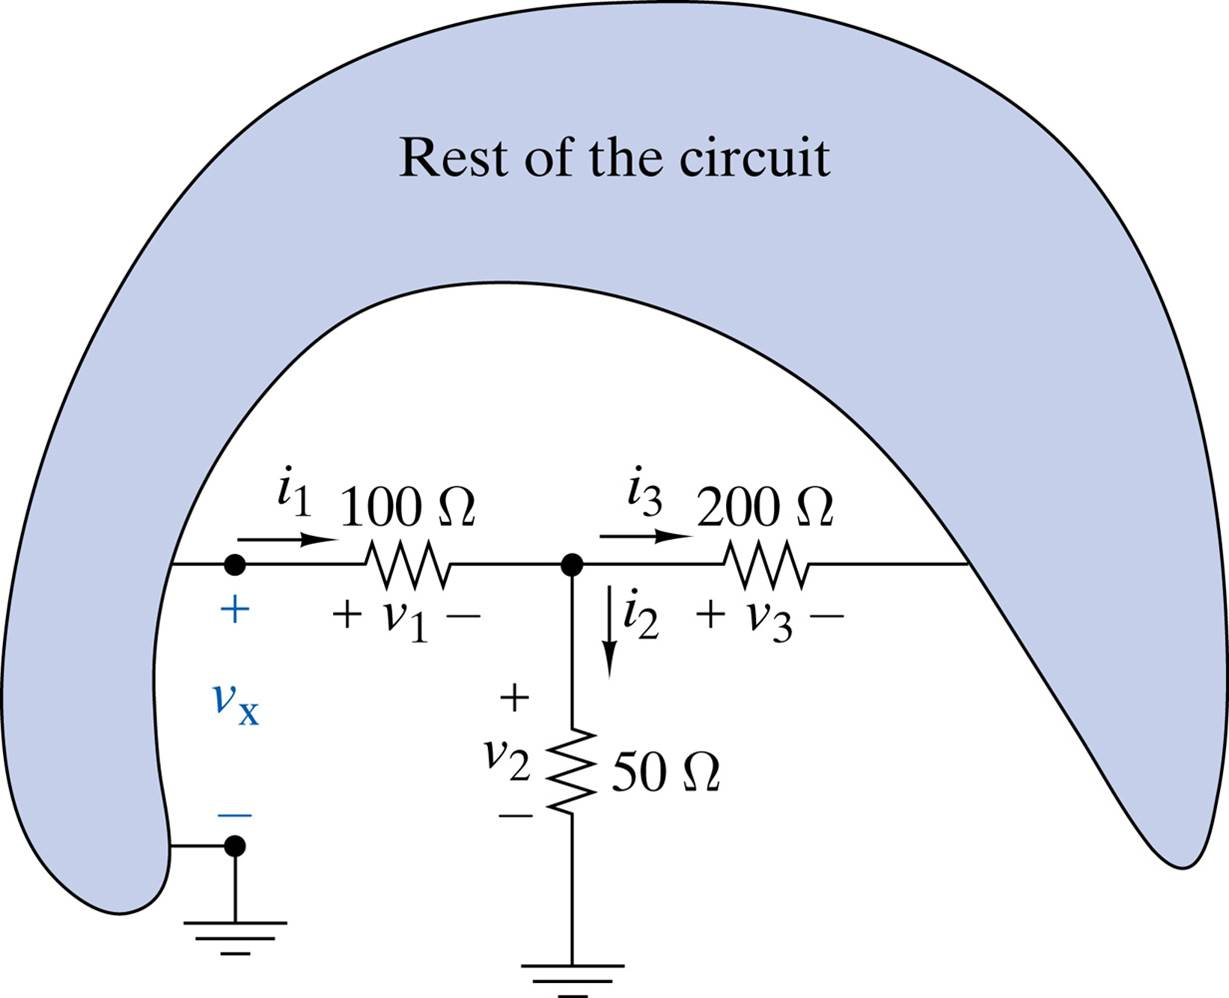
\includegraphics[width=0.5\textwidth]{KCL.jpg}
\caption{KCL Example}
\label{fig: KCL}
\end{figure}

\soln{1in}{
\begin{eqnarray}
i_1-i_2-i_3 = 0 \\
i_1 = i_2+i_3 \nonumber
\end{eqnarray}
}


\newpage
\textbf{KCL Example}---This is problem 2-20 from the textbook.

\begin{figure}[h b t]
\centering
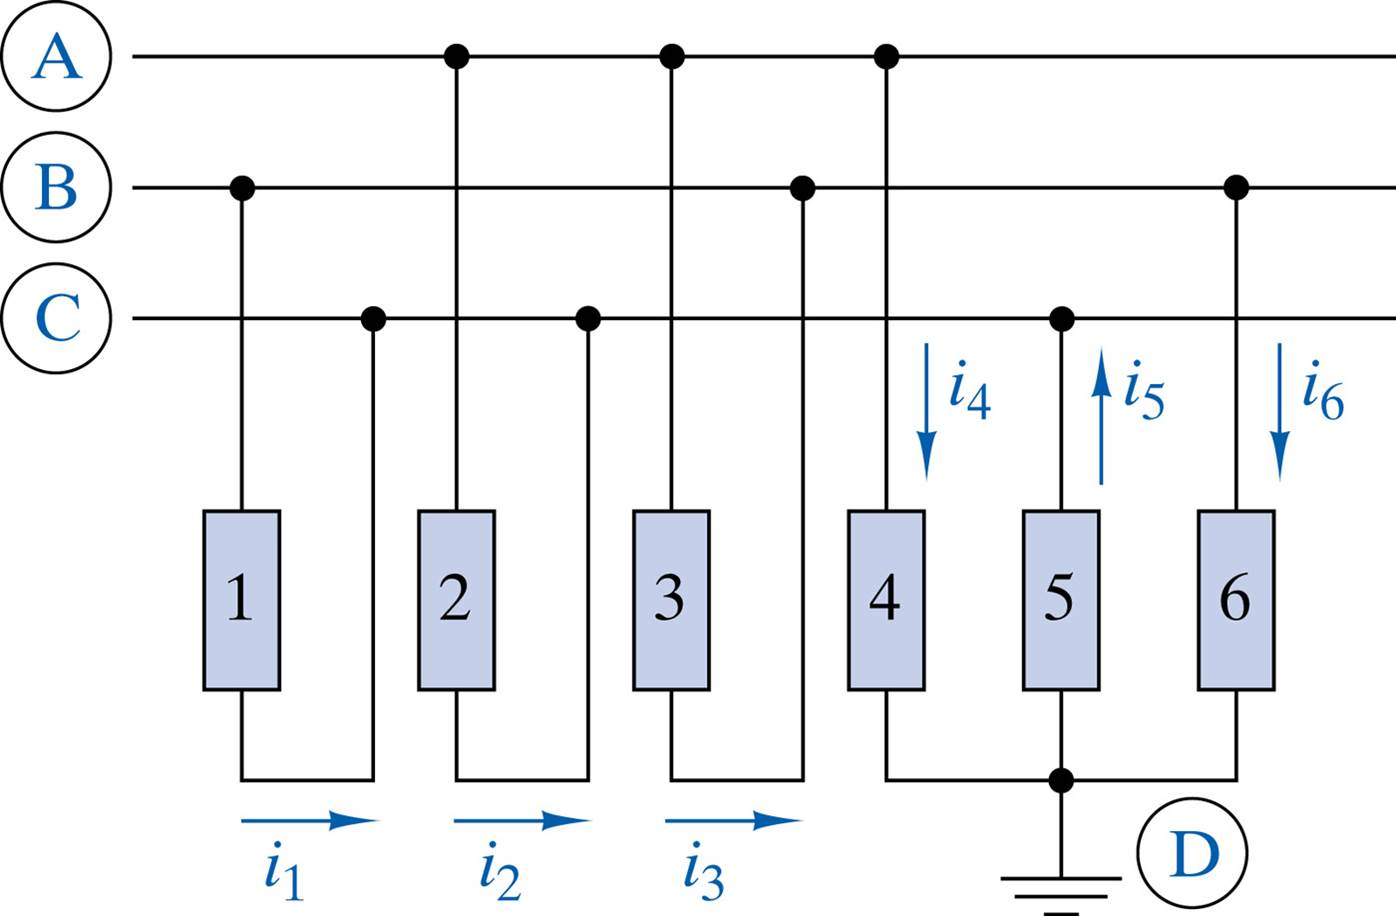
\includegraphics[width=0.5\textwidth]{KCL_Example.jpg}
\caption{A second KCL Example}
\label{fig: KCL_Example}
\end{figure}

The circuit in Figure \ref{fig: KCL_Example} is organized around 3 signal lines A, B \& C (assume lines are open circuits off both edges). 
\begin{itemize}
\item How many nodes are in this circuit?
\item Write KCL equations for the circuit
\item If $i_1 = -20\ mA$, $i_2 = -12\ mA$, and $i_3 = 50\ mA$; find $i_4$, $i_5$, \& $i_6$
\end{itemize}

\soln{6in}{
There are 4 nodes in this circuit (each signal line and the ground)

KCL equations are:
\begin{eqnarray}
i_2+i_3+i_4=0 \nonumber \\
i_3 = i_1+i_6 \\
i_1+i_2+i_5=0 \nonumber \\
i_4+i_6=i_5 \nonumber 
\end{eqnarray}

We can use $i_1$ and $i_2$ to find $i_5$
\begin{eqnarray}
i_5&=&-(i_1+i_2) \nonumber \\
i_5&=&-(-20\ mA+ (-12\ mA)) \nonumber\\
i_5&=&32\ mA \nonumber
\end{eqnarray}

We can use  $i_2$ and $i_3$ to find $i_4$
\begin{eqnarray}
i_4&=&-(i_2+i_3) \nonumber \\
i_4&=&-(-12\ mA+ 50\ mA) \nonumber\\
i_4&=&-38\ mA \nonumber
\end{eqnarray}

We can use  $i_4$ and $i_5$ to find $i_6$
\begin{eqnarray}
i_6&=&i_5-i_4 \nonumber \\
i_6&=&32\ mA - (-38\ mA) \nonumber\\
i_6&=&70\ mA \nonumber
\end{eqnarray}
}

What you may have noticed in our solution above was that we were able to write 4 KCL equations; one for each node.  What may not be obvious is that only 3 of the equations were linearly independent.  The proof of this is below:


We can rewrite our 4 equations in matrix form

\soln{5in}{
\begin{equation} \nonumber
\left [\begin{array}{rrrrrr}
0 & -1 & -1 & -1 & 0 & 0 \\
-1 & 0 & 1 & 0 & 0 & -1 \\
1 & 1 & 0 & 0 & 1 & 0 \\
0 & 0 & 0 & 1 & -1 & 1 \\
\end{array} \right ]
\left [\begin{array}{r}
i_1\\  i_2 \\ i_3 \\  i_4 \\ i_5 \\  i_6
\end{array}\right ] = 
\left [ \begin{array}{c}
0 \\ 0 \\ 0 \\0
\end{array} \right ]
\end{equation}

If we focus on just the coeffcient matrix, we can use row reduction techniques to rewrite the matrix as

\begin{equation} \nonumber
\left [\begin{array}{rrrrrr}
1 & 1 & 0 & 0 & 1 & 0 \\
0 & 1 & 1 & 1 & 0 & 0 \\
0 & 0 & 0 & 1 & -1 & 1 \\
0 & 0 & 0 & 0 & 0 & 0 \\
\end{array} \right ]
\end{equation}

The fact that the matrix can be row-reduced to give a zero row tells you that one of the equations is not linearly independent.

}

\newpage


\section{Kirchhoff's Voltage Law (KVL)}
Kirchhoffs Voltage Law in words:
\soln{1.5in}{
\begin{enumerate}
\item The algebraic sum of voltages around any closed path equals zero
\item The sum of voltage rises around a loop equals the sum of voltage drops around the same loop
\item If it goes up, it must come down
\end{enumerate}
}

KVL in mathmatics:
\begin{equation}
\sum_{Loop} v = 0 
\end{equation}

\begin{equation}
\sum v_{rises} = \sum v_{losses}
\end{equation}

\textbf{KVL Example 1:} Write KVL equations (for the two labeled loops) and find unknown voltages for the circuit shown in Figure \ref{fig: KVL_Example_1}.  [Exercise 2-5 from text]

\begin{figure}[h b t]
\centering
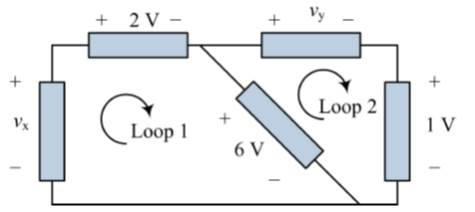
\includegraphics[width=0.5\textwidth]{KVL_Example_1.jpg}
\caption{A KVL Example}
\label{fig: KVL_Example_1}
\end{figure}

\soln{2.5in}{
We start by writing the KVL equations.

Loop 1:
\begin{equation}
v_x-2\ V - 6\ V = 0
\end{equation}

Loop 2
\begin{equation}
6\ V - v_y - 1\ V= 0
\end{equation}

We can now solve each equation to see that $v_x=8\ V$ and $v_y = 5\ V$. 
}

\newpage
\pagebreak
\clearpage

\textbf{KVL Example 2:} Find $v_x$, $v_y$, and $v_z$ in the circuit shown in Figure \ref{fig: KVL_Example_2}. [Exercise 2-6 from text]. This example is a little unique in that we are going to define a loop where one does not physically exist. 

\begin{figure}[h b t]
\centering
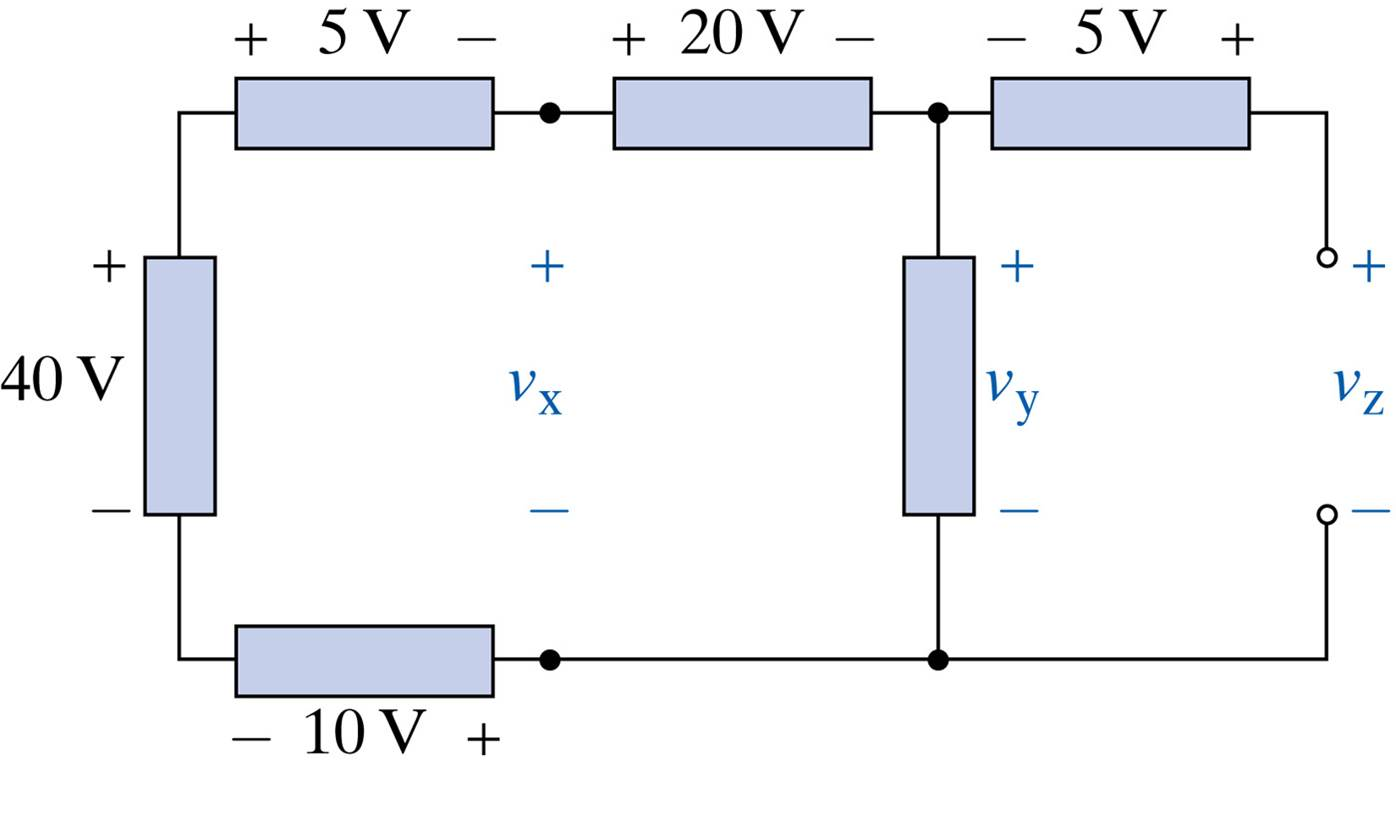
\includegraphics[width=0.4\textwidth]{KVL_Example_2_unlabeled_loops.jpg}
\caption{A second KVL Example}
\label{fig: KVL_Example_2}
\end{figure}

\begin{figure}[h b t]
\centering
\soln{2.5}{
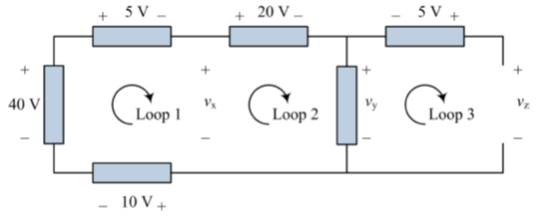
\includegraphics[width=0.5\textwidth]{KVL_Example_2_labeled_loops.jpg}
}
\caption{Circuit above with loops labeled}
\label{fig: KVL_Example_2_loops}
\end{figure}

\soln{4in}{
To start the problem lets label some loops... This is the tricky part. Notice we defined 2 loops inside a ``single loop''.  Because we defined $v_x$ the way we did, we can account for this rise/loss in each ``loop''.


Next we write the KVL equations.

Loop 1:
\begin{equation}
40\ V - 5\ V- v_x - 10\ V=0
\end{equation}

Loop 2
\begin{equation}
v_x -20\ V-v_y=0
\end{equation}

Loop 3
\begin{equation}
v_y + 5\ V - v_z = 0
\end{equation}

We can now solve each equation to see that $v_x=25\ V$, $v_y = 5\ V$, and $v_z = 10\ V$. 
}

\newpage
\pagebreak
\clearpage

\section{Review Questions}
\begin{questions}
\item What does it really mean is we calculate a negative voltage or current?

\soln{1in}{When we get a negative number for voltage or current, it just means our initial ``assigned'' voltage polarity or current direction was wrong.  You can flip the polarity/direction and drop the negative.}

\item What is the current through an open circuit?

\soln{1in}{Zero}

\item What is the voltage across a short circuit?

\soln{1in}{Zero, there is not voltage across a short circuit.  Since voltage is measure between two nodes and a short circuit does not seperate any nodes, you cannot measure a voltage across it.}

\newpage


\end{questions}

\end{document}


% Equation Array Example Code
%\begin
%{eqnarray}
%P_R &=& i_R^2R \nonumber \\
%P_R &=& (100\ mA)^2 \times 100\ \Omega \nonumber \\
%P_R &=& (100 \times 10^{-3}\ A)^2 \times 100\ \Omega \\
%P_R &=& 10000 \times 10^{-6}\ A^2  \times 100\ \Omega \nonumber \\
%P_R &=& 1\ W  \nonumber
%\end{eqnarray} 

% Figure Example Code
%\begin{figure}[h b t]
%\centering
%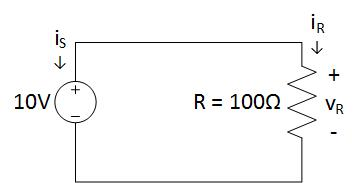
\includegraphics[width=0.5\textwidth]{OhmsLawExampleSolution.jpg}
%\caption{Ohm's Law example circuit}
%\label{fig: OhmsLawExampleSolution}
%\end{figure}

%Table Example Code
%\begin{table}[h b t]
%\centering
%\begin{tabular}{|l|c|c|}
%\hline
%Prefix & Abbreviation & Value \\
%\hline \hline
%Giga & $G$ & $10^9$ \\
%Mega & $M$ & $10^6$ \\
%Kilo & $k$ & $10^3$ \\
%\hline
%milli & $m$ & $10^{-3}$ \\
%micro & $\mu$ & $10^{-6}$ \\
%nano & $n$ & $10^{-9}$ \\
%pico & $p$ & $10^{-12}$ \\
%\hline
%\end{tabular}
%\caption{Engineering prefixes and values}
%\label{tab: Eng Prefixes}
%\end{table}
